\documentclass{standalone}
\usepackage{tikz}
\begin{document}
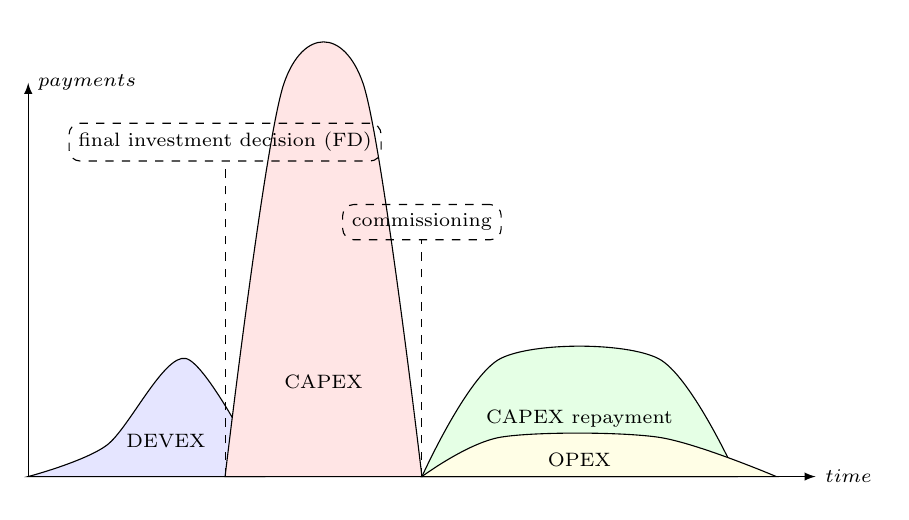
\begin{tikzpicture}[every node/.style={font=\scriptsize}]
    \draw[->,>=latex] (0,0) -- (10,0) node[right] {$time$};
    \draw[->,>=latex] (0,0) -- (0,5) node[right] {$payments$};

    \draw[fill=blue!10,smooth] plot coordinates {(0,0) (1,0.4) (2,1.5) (3,0)} -- cycle;
    \node[above] at (1.75,0.25) {DEVEX} ;

    \draw[fill=red!10,smooth] plot coordinates {(2.5,0) (3.25,5) (4.25,5) (5,0)} --  cycle;
    \node[above] at (3.75,1) {CAPEX} ;
    
    \draw[fill=green!10,smooth] plot coordinates {(5,0) (6,1.5) (8,1.5) (9,0)} --  cycle;
    \node[above] at (7,0.5) {CAPEX repayment} ;

    \draw[fill=yellow!10,smooth] plot coordinates {(5,0) (6,0.5) (8,0.5) (9.5,0)} --  cycle;
    \node[above] at (7,0) {OPEX} ;
    
    \draw[dashed] (2.5,0) -- (2.5,4) node [above,draw, rounded corners] {final investment decision (FD)};
    
    \draw[dashed] (5,0) -- (5,3) node [above,draw, rounded corners] {commissioning};
    
\end{tikzpicture}
\end{document}